%
% File coling2020.tex
%
%% Based on the style files for COLING-2018
%

\documentclass[11pt]{article}
\usepackage{coling2020}
\usepackage{times}
\usepackage{url}
\usepackage{latexsym}

\setlength\titlebox{4cm}
\colingfinalcopy

\title{Image Processing and Computer Vision \\[1ex] COMS30031}

\author{
    Kai Hulme \\
    kh16747 \\
    University of Bristol \\
    26th July 2021 \\
}

\begin{document}

\maketitle
\newpage

\section{Face Detection with Viola-Jones}
\label{vj_object_detector}

\subsection{Ground Truth and Detection Visualisation}

% Manually annotate all the test images and generate ground truth in form of bounding box $(x,y,width,height)$ coordinates for all valid frontal faces and store these annotations (e.g. in a file or array). Then test the detector’s performance (with the given parameters as provided by $face.cpp$) on five given example images: $dart4.jpg$, $dart5.jpg$, $dart13.jpg$, $dart14.jpg$ and $dart15.jpg$. Produce the five result images with bounding boxes of the ground truth (in red) and actually detected instances (in green) drawn around frontal faces and include them in your report.  

% Implement some code using a manually fixed threshold on the Intersection-Over-Union (IOU) between bounding boxes to judge which faces given the ground truth were successfully detected. Calculate and note in your report in table form the TPR (true positive rate) for all test images, that is the fraction of successfully detected faces out of all valid faces in an image.

% Discuss briefly in your report:
%     - some practical difficulties in assessing the TPR meaningfully
%     - why it is always possible to achieve a TPR of 100\% on any detection  task, and  
%     - implement  a  small  piece  of  code  to calculate the $F_1$-score of your face detection system  accurately and meaningfully for all test images given the ground truth and include it as a table in the report.

\begin{figure}[h]
\centering
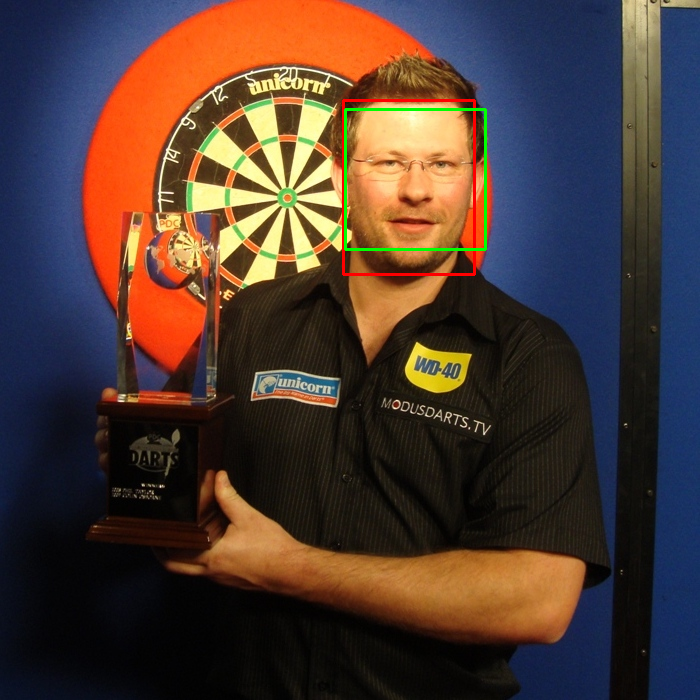
\includegraphics[height=0.16\textwidth]{figures/01_vj_faces/dart4_true_pred_vj_face.png}
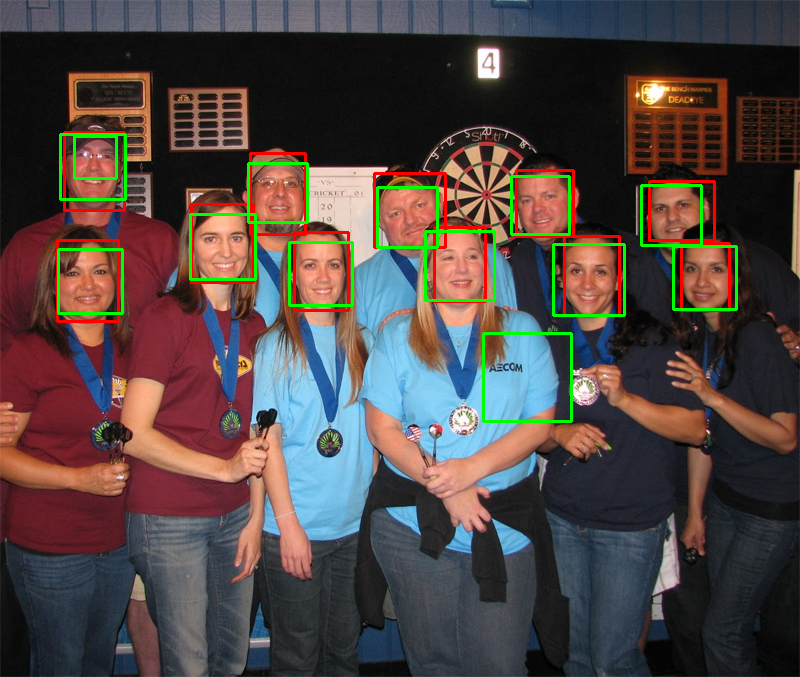
\includegraphics[height=0.16\textwidth]{figures/01_vj_faces/dart5_true_pred_vj_face.png}
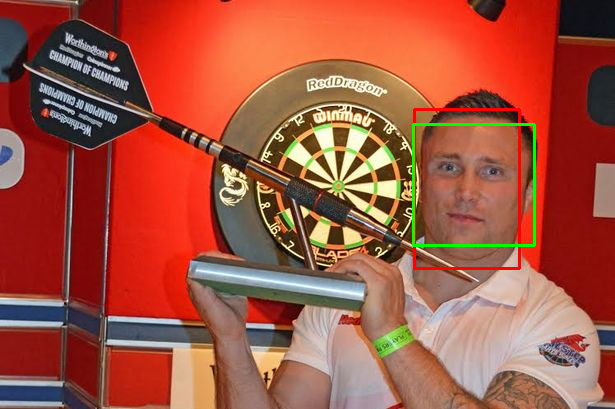
\includegraphics[height=0.16\textwidth]{figures/01_vj_faces/dart13_true_pred_vj_face.png} \\ [0.3ex]
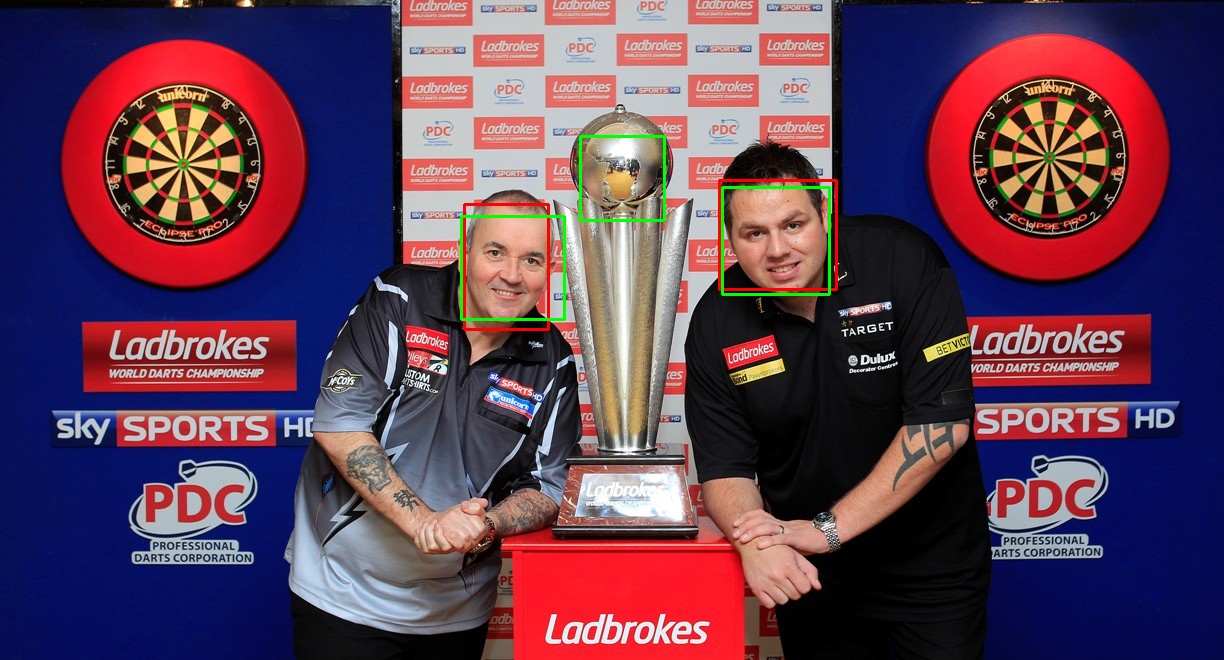
\includegraphics[height=0.16\textwidth]{figures/01_vj_faces/dart14_true_pred_vj_face.png}
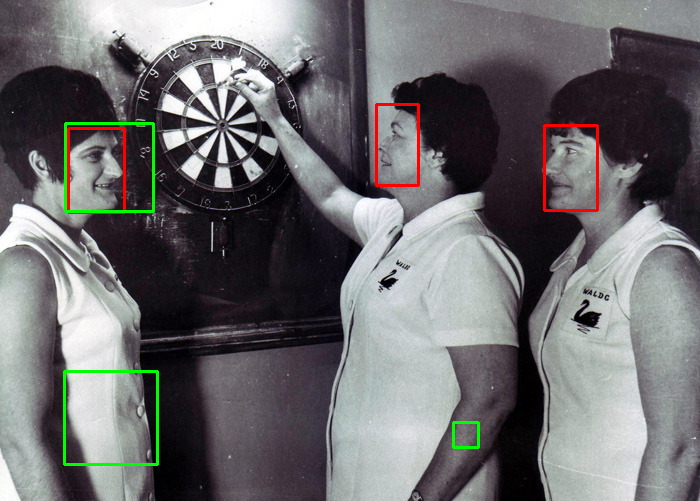
\includegraphics[height=0.16\textwidth]{figures/01_vj_faces/dart15_true_pred_vj_face.png}
\caption{Results of Viola-Jones face detection on images $dart4.jpg$, $dart5.jpg$, $dart13.jpg$, $dart14.jpg$ and $dart15.jpg$ (from top-left to bottom-right), with ground truth bounding boxes in red and detections in green. Performance on the top row of images is perfect, with no false positives (FP) or false negatives (FN). The lower-left image has detected both faces but has mistakenly detecting the trophy as a face. The lower-right image has detected the face of the most forward facing woman but has missed the two on the right who are at a greater angle to the camera, indicating it struggles to detect less straight-on faces - likely due to less facial features being visible.}
\label{vj_faces_images}
\end{figure}

\subsection{IoU, Precision, Recall and $F_1$-Score}

\begin{minipage}{.19\linewidth}
\begin{equation}
\centering
IoU_{a,b} = \frac{A_{a \cap b}}{A_{a \cup b}}
\end{equation}
\end{minipage} 
\begin{minipage}{.26\linewidth}
\begin{equation}
precision = \frac{TP}{TP + FP}
\end{equation}
\end{minipage}
\begin{minipage}{.23\linewidth}
\begin{equation}
recall = \frac{TP}{TP + FN}
\end{equation}
\end{minipage}
\begin{minipage}{.3\linewidth}
\begin{equation}
\centering
F_1 = \frac{2 \cdot precision \cdot recall}{precision + recall}
\end{equation}
\end{minipage}
\\ [2ex]

\begin{wraptable}{r}{5.5cm}
\begin{tabular}{|c||c|c|c|} 
     \hline
     Image & Precision & Recall & $F_1$ \\ [0.5ex] 
     \hline
     $dart0$  & 1.00  & 1.00  & 1.00  \\ 
     $dart1$  & $n/a$ & $n/a$ & $n/a$ \\ 
     $dart2$  & $n/a$ & $n/a$ & $n/a$ \\ 
     $dart3$  & $n/a$ & $n/a$ & $n/a$ \\ 
     $dart4$  & 1.00  & 1.00  & 1.00  \\ 
     $dart5$  & 0.85  & 1.00  & 0.92  \\  
     $dart6$  & 0.00  & 0.00  & 0.00  \\  
     $dart7$  & 1.00  & 1.00  & 1.00  \\  
     $dart8$  & 0.00  & 0.00  & 0.00  \\ 
     $dart9$  & 1.00  & 1.00  & 1.00  \\ 
     $dart10$ & $n/a$ & $n/a$ & $n/a$ \\ 
     $dart11$ & 1.00  & 1.00  & 1.00  \\  
     $dart12$ & $n/a$ & $n/a$ & $n/a$ \\ 
     $dart13$ & 1.00  & 1.00  & 1.00  \\  
     $dart14$ & 0.67  & 1.00  & 0.80  \\  
     $dart15$ & 0.33  & 0.33  & 0.33  \\ [1ex] 
     \hline
\end{tabular}
\caption{Table showing detection performance of Viola-Jones for each test image. $n/a$ entries indicate no faces in test image which would result in undefined precision, recall and $F_1$ metrics.}
\label{vj_faces_results}
\end{wraptable} 

When evaluating an object detector we are interested in its ability to correctly detect what we are looking for, e.g. faces. A correct detection is a true positive (TP), a false detection is a false positive (FP) and a missed detection is a false negative (FN). To check if a detection is correct, the detected bounding box is compared to the ground truth bounding using the Intersection over Union (IoU) $(1)$. Non-intersecting boxes give an IoU of 0 (as $A_{a \cap b}=0$) and 1 for perfectly intersecting boxes (as $A_{a \cap b}=A_{a \cup b}$); a detection is correct if the IoU of the detection and ground truth is greater than some threshold value.

{\color{white}.}

Recall $(3)$, also called the true positive rate, measures the proportion of positive detections out of all the positives, effectively measuring the detectors ability to detect. However, recall alone should not determine the performance of a detector. A na\"ive detector could return every possible bounding box which would include the ground truths, but this would not be of use as there are so many FPs. Precision $(2)$ measures the proportion of correct detections from all of the detections. A precise detector will still aim to find TPs, but reduce FPs. $F_1$-score $(4)$ is the harmonic mean of precision and recall, meaning a detector with a high $F_1$ will have both high precision and recall which should result in accurate detections with few mistakes. Table \ref{vj_faces_results} shows the precision, recall and $F_1$-score of the face detection results from the Viola-Jones cascade detector on each of the test images.

{\color{white}.}

Recall (or TPR) cannot be measured accurately when there is nothing to detect. Looking at $(3)$, if there are no true positives or detections precision is undefined. For example: with $TP = 0$ and $FN = 0$, $recall = \frac{0}{0+0}$. For this \\ reason images with no faces in Table \ref{vj_faces_results} have $n/a$ results.

\newpage

\section{Dartboard Detection with Viola-Jones}
\label{own_detector}

\subsection{Training Performance}
\label{training_performance} 

% The training tool produces a strong classifier in stages. Per stage the tool adds further features to the classifier and prints the achieved TPR and FPR (false positive rate) for that point on the training data (see Figure). Collate this information into a graph that plots TPR vs FPR on the training data for the three different stages. Produce this graph in your report and briefly interpret what it shows. 

\begin{figure}[h]
\floatbox[{\capbeside\thisfloatsetup{capbesideposition={right,top},capbesidewidth=9cm}}]{figure}[\FBwidth]
{\caption{True positive rate (TPR) and false positive rate (FPR) throughout 3 stages of training Viola-Jones cascade for dartboard detection. The Viola Jones algorithm is trained in a number of stages. At each stage a new layer will be added to the detector in the form of a cascade. The training results indicate the cascade favours maximising detections first, giving a TPR close to $1.00$ at the expense of the FPR being $1.00$ As training progresses the cascade becomes more precise with the FPR dropping close to $0.00$ by stage 3. The final cascade will have a high $F_1$ close to $1.00$ when tested on the training images.}}
{\fbox{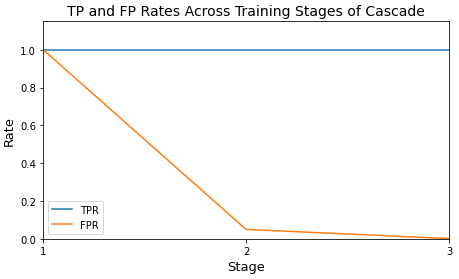
\includegraphics[height=0.3\textwidth]{figures/02_vj_dartboards/cascade_training_tpr_fpr.png}}}
\label{training_tpr_fpr}
\end{figure}

\subsection{Testing Performance}

% Test  the  dartboard  detector’s performance on all given example images. Produce the result images with bounding boxes drawn around detected dartboard candidates (in green) and ground truth (in red) and include 3 of them in your report. In tabular form, calculate the overall TPR and $F_1$ score per image and the average  of these scores across the 16 images. Briefly discuss the performance achieved and give reasons for the different TPR values compared to the performance achieved in a).

\begin{figure}[h]
\centering
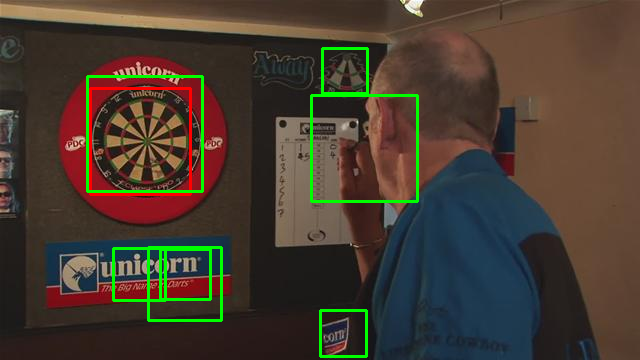
\includegraphics[height=0.18\textwidth]{figures/02_vj_dartboards/dart2_true_pred_vj_dartboards.png}
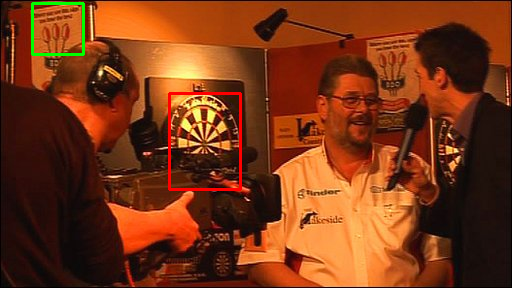
\includegraphics[height=0.18\textwidth]{figures/02_vj_dartboards/dart11_true_pred_vj_dartboards.png}
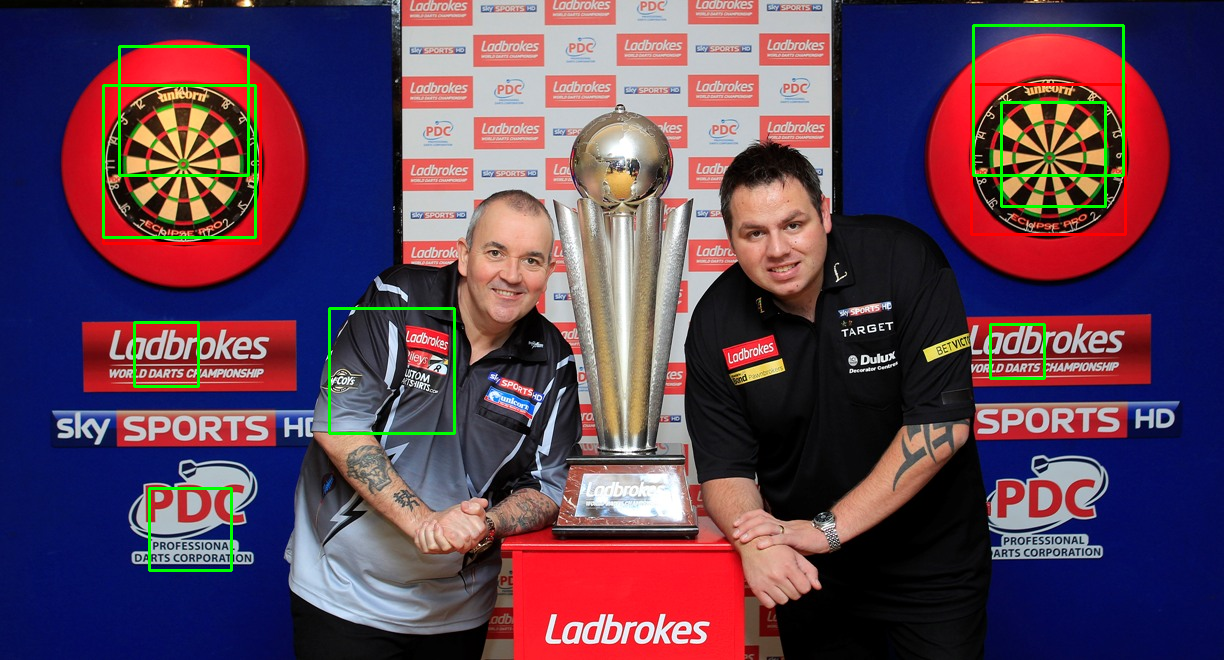
\includegraphics[height=0.18\textwidth]{figures/02_vj_dartboards/dart14_true_pred_vj_dartboards.png}
\caption{Results of Viola-Jones dartboard detection on images $dart2.jpg$, $dart11.jpg$, $dart14.jpg$ (from left to right), with ground truth bounding boxes in red and detections in green.}
\label{vj_dartboards_images}
\end{figure}

\FloatBarrier

% \begin{table}[h]
\begin{wraptable}{r}{5.5cm}
\begin{tabular}{|c||c|c|c|} 
     \hline
     Image & Precision & Recall & $F_1$ \\ [0.5ex] 
     \hline
     $dart0$  & 1.00 & 1.00 & 1.00 \\ 
     $dart1$  & 0.50 & 1.00 & 0.67 \\ 
     $dart2$  & 0.14 & 1.00 & 0.25 \\ 
     $dart3$  & 0.33 & 1.00 & 0.50 \\ 
     $dart4$  & 1.00 & 1.00 & 1.00 \\ 
     $dart5$  & 0.20 & 1.00 & 0.33 \\  
     $dart6$  & 1.00 & 1.00 & 1.00 \\  
     $dart7$  & 0.50 & 1.00 & 0.67 \\  
     $dart8$  & 0.20 & 0.50 & 0.29 \\ 
     $dart9$  & 0.25 & 1.00 & 0.40 \\ 
     $dart10$ & 0.43 & 1.00 & 0.60 \\ 
     $dart11$ & 0.00 & 0.00 & 0.00 \\
     $dart12$ & 1.00 & 1.00 & 1.00 \\  
     $dart13$ & 0.50 & 1.00 & 0.67 \\  
     $dart14$ & 0.25 & 1.00 & 0.40 \\  
     $dart15$ & 1.00 & 1.00 & 1.00 \\
     \hline\hline
     avg.  & 0.52 & 0.90 & 0.61 \\
     \hline
\end{tabular}
\caption{Dartboard detection performance of Viola-Jones method for each image and overall}
\label{vj_dartboards_results}
% \end{table}
\end{wraptable} 

Figure \ref{vj_dartboards_images} shows the detections made by the Viola-Jones cascade trained to detect dartboards. Ground truth bounding boxes are shown in red and the cascade's predictions are shown in red. I used a threshold of $0.5$ for the IoU between the boxes to discern TPs from FPs.

{\color{white}.}

Looking at the first image we can see the Viola-Jones method has detected the target dartboard well, but there are a large number of FPs resulting in a recall of $1.00$, but a precision of only $0.14$ giving an $F_1$ of $0.25$. The second image shows a missed detection (FN), likely caused by the dartboard being obstructed by camera, there is also a FP in the upper-right corner giving an $F_1$ of $0.0$. The image on the right shows the system is able to detect multiple dartboards. However, not only are there are FP detections, but the dartboards have been detected multiple times (multiple detections are FPs), meaning while \\ recall is $1.00$, precision is $0.25$.

{\color{white}.}    

Overall it seems the Viola-Jones method works well for non-obstructed dartboards. However the system has many FPs and its precision and consequently its $F_1$ suffers from this. Testing gives a high recall of $0.90$, but a low precision and $F_1$ of $0.52$ and $0.61$ respectively. When improving this system I aim to increase the precision whilst trying to retain its high recall. 

{\color{white}.}

The testing results in Table \ref{vj_dartboards_results} differ from those seen during training in Figure \ref{training_tpr_fpr}. This indicates the Viola-Jones method has some degree of overfitting to the training data and so performance suffers when tested on unseen data. This is likely due to the nature of the training data differing from the test data; the positive samples in training were all augmentations of the same dartboard; where the testing data is more varied with different board types, lighting conditions, obstructions which lead to FNs, as well as other items in the image which lead to FPs.

\newpage

\section{Integration with Shape Detectors}

\subsection{Hough Details}
\label{hough_details}

\begin{figure}[h]
\centering
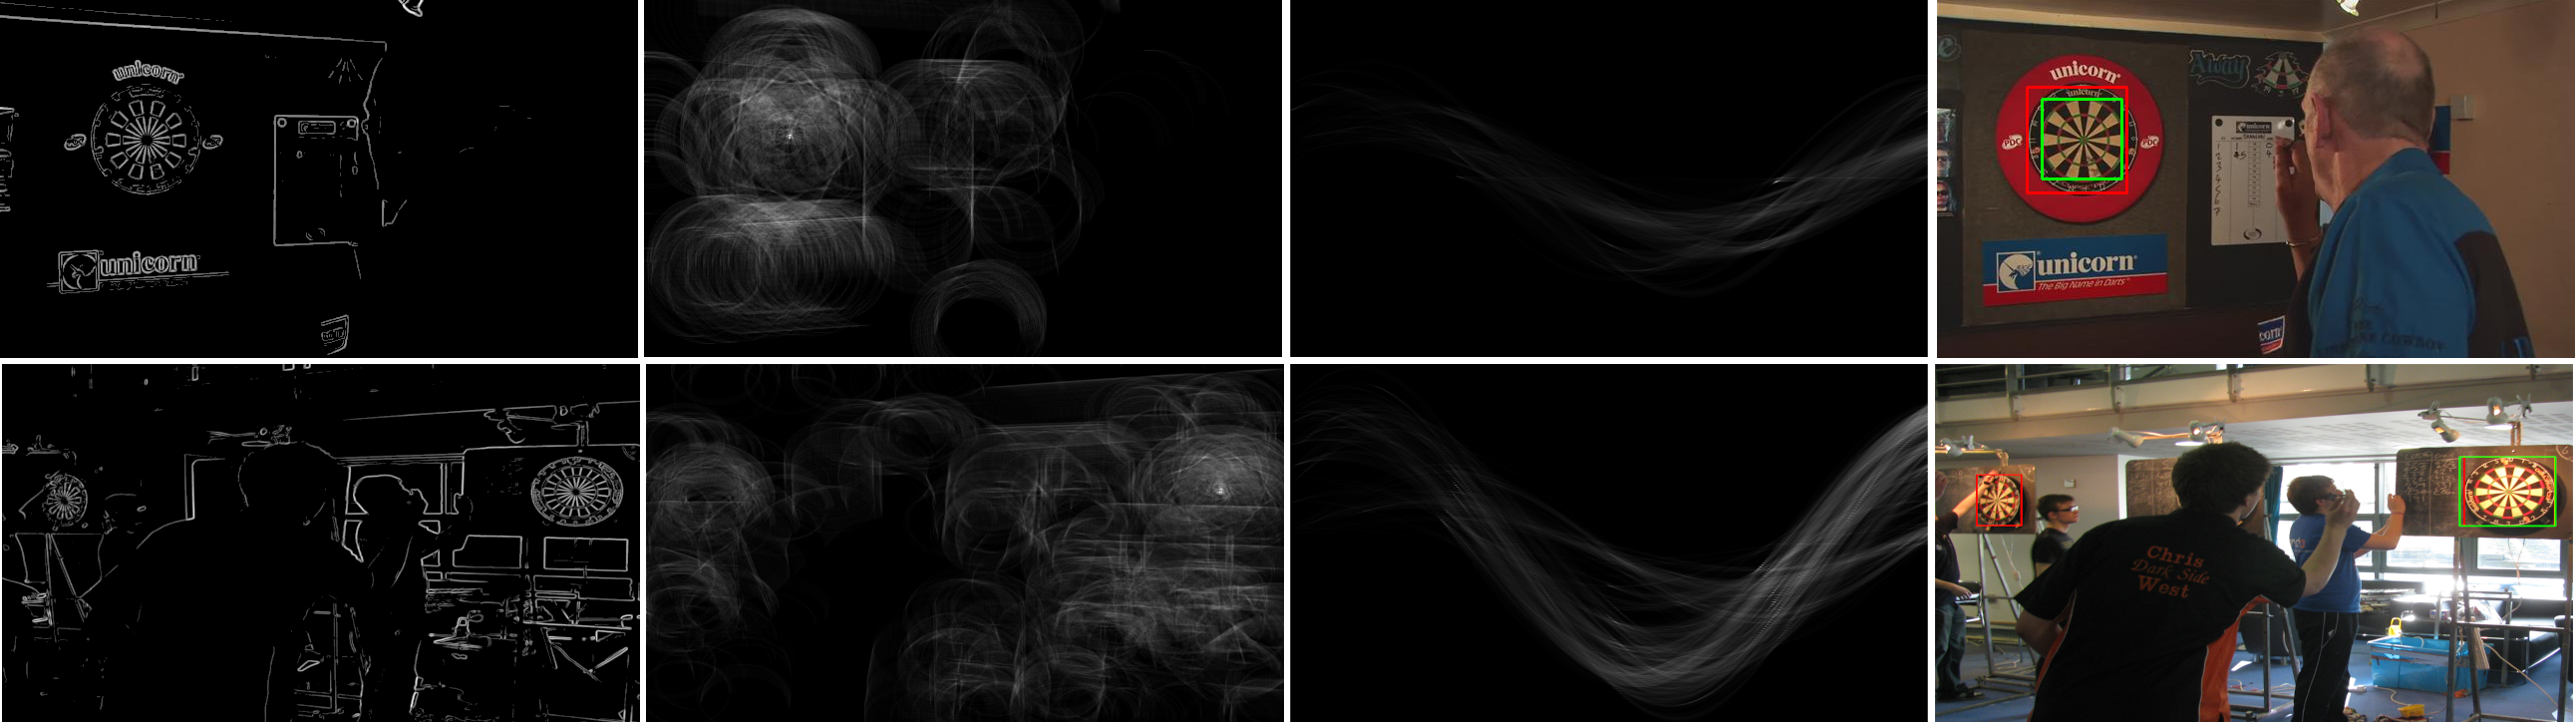
\includegraphics[width=0.95\linewidth]{figures/03_shape_detection/shape_detection_results.png}
\caption{Thresholded gradient magnitude from Sobel edge detection, Hough (circles) space at radius close to ground truth, Hough (lines) space and detections for $dart2$ (top row) and $dart8$ (bottom row). Images have been resized.}
\label{hough_images}
\end{figure}

\subsection{Evaluation}

\begin{wraptable}{r}{8.5cm}
% \begin{table}[h]
\begin{tabular}{|c||c|c|c|} 
    \hline
    Image & Precision & Recall & $F_1$ \\ [0.5ex] 
    \hline
    $dart0$  & 1.00 (+0.00) & 1.00 (+0.00) & 1.00 (+0.00) \\
    $dart1$  & 1.00 (+0.05) & 1.00 (+0.00) & 1.00 (+0.33) \\
    $dart2$  & 1.00 (+0.86) & 1.00 (+0.00) & 1.00 (+0.75) \\
    $dart3$  & 0.00 (-0.33) & 0.00 (-1.00) & 0.00 (-0.50) \\
    $dart4$  & 1.00 (+0.00) & 1.00 (+0.00) & 1.00 (+0.00) \\
    $dart5$  & 0.00 (-0.20) & 0.00 (-1.00) & 0.00 (-0.33) \\
    $dart6$  & 0.00 (-1.00) & 0.00 (-1.00) & 0.00 (-1.00) \\
    $dart7$  & 1.00 (+0.50) & 1.00 (+0.00) & 1.00 (+0.33) \\
    $dart8$  & 1.00 (+0.80) & 0.50 (+0.00) & 0.67 (+0.38) \\
    $dart9$  & 0.50 (+0.25) & 1.00 (+0.00) & 0.67 (+0.27) \\
    $dart10$ & 1.00 (+0.57) & 0.67 (-0.33) & 0.80 (+0.20) \\
    $dart11$ & 0.00 (+0.00) & 0.00 (+0.00) & 0.00 (+0.00) \\
    $dart12$ & 1.00 (+0.00) & 1.00 (+0.00) & 1.00 (+0.00) \\
    $dart13$ & 1.00 (+0.50) & 1.00 (+0.00) & 1.00 (+0.33) \\
    $dart14$ & 0.67 (+0.42) & 1.00 (+0.00) & 0.80 (+0.40) \\
    $dart15$ & 1.00 (+0.00) & 1.00 (+0.00) & 1.00 (+0.00) \\
    \hline\hline
    avg.     & 0.70 (+0.18) & 0.70 (-0.20) & 0.70 (+0.09) \\
    \hline
\end{tabular}
\caption{Dartboard detection performance of ensemble method for each image and overall with improvements over Viola-Jones method shown for each entry.}
\label{ensemble_dartboards_results}
% \end{table}
\end{wraptable} 

% Evaluate your detector on all of the example images. Provide the TPR and $F_1$-score for each of the test images and their average across the 16 images in a table. Note in extra table columns the difference w.r.t. to the detection performances using only the Viola-Jones detector. Briefly note in bullet points the key merits and shortcomings of your now enhanced implementation.

% Table \ref{ensemble_dartboards_results} shows the dartboard detection results for my \\ ensemble method.

• Looking at Figure \ref{hough_images} my ensemble method was able to detect boards where the Viola-Jones method missed, whilst greatly reducing the number of FPs.

% {\color{white}.}

\noindent • Table \ref{ensemble_dartboards_results} shows a precision increase of 0.18 due to far less FPs. The detection rate suffered but the Viola-Jones method had such a high recall due to its low precision; if you say everything is a dartboard you'll not miss any.

% {\color{white}.}

\noindent • Overall the system had an increase in $F_1$ score whilst being far more precise than the Viola-Jones method alone. Further improvements will aim to increase the recall.

\subsection{Detection Pipeline}

% In a flow diagram, depict how you have combined evidence from the Hough Transform(s) and Viola-Jones detector. In bullet points, explain briefly your rationale behind the way you have combined evidence.  

% Figure \ref{detection_pipeline} shows the data pipeline for dartboard detection with my system.

% {\color{white}.}

\noindent • As my aim was to create a more precise system I decided to use an ensemble of detectors and require two methods to agree on a detection before accepting it.

% {\color{white}.}

\noindent • The 3 methods are the original Viola-Jones cascade along with circle and line detection via Hough transforms.

% {\color{white}.}

\noindent • Dartboards are circular with lines separating scoring zones, so a circle with enough lines passing through must be a dartboard. Checking if a Viola-Jones detection has either a circle centre or enough lines passing through would also result in a detection.

% {\color{white}.}

\noindent • Additional checks were added to ensure each dartboard was only detected once. 

\begin{figure}[b]
\centering
\fbox{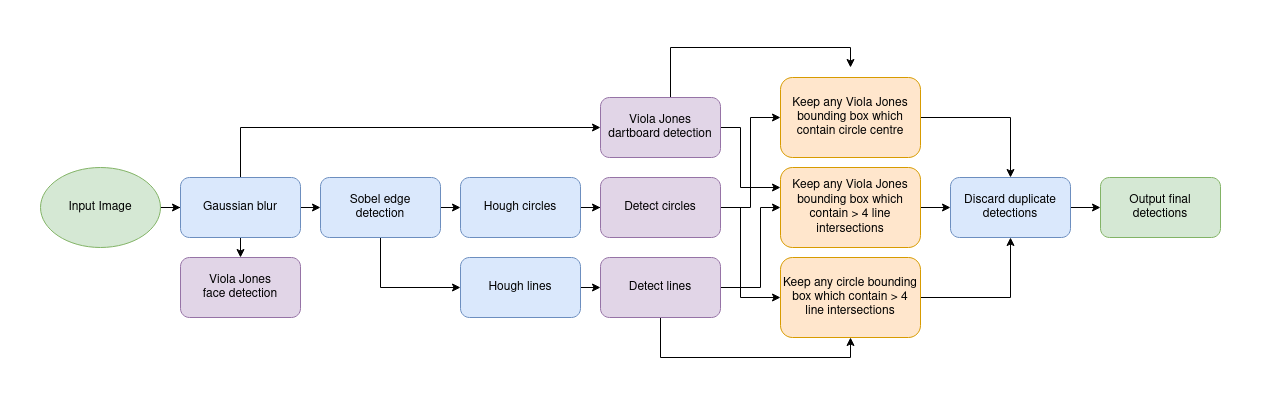
\includegraphics[width=0.9\textwidth]{figures/03_shape_detection/object_detection_pipeline.png}}
\caption{Flow diagram depicting ensemble method of Viola-Jones with Hough transforms for dartboard detection.}
\label{detection_pipeline}
\end{figure}

\newpage

\section{Improving my Detector}
\label{detector_improvements}

\subsection{Idea and Visualisation}
\label{idea_vis}

% {\color{blue}
% In bullet points, explain briefly your rationale behind selecting the approach you have taken. 
% } \\

• The first improvement I made was to the Hough transforms; using gradient angles obtained during Sobel edge detection I reduced the range of angles used to increment the accumulator for both Hough lines and circles. This reduced the amount of noise within the Hough space caused by intersections of points of non-interest accumulating to high values which result in FPs. Figure \ref{detector_improvement_images} shows this reduction in noise resulting in an accurate circle detection. This method greatly increased precision but I included the results with the previous section in Table \ref{detector_improvement_images}.

\noindent • The second improvement was to cluster the colours of the image using KMeans. When inspecting some of the images I noticed many FP detected circles; Figure \ref{detector_improvement_images} shows this in $dart3.jpg$. Using color segmentation I hoped problem areas would be segmented together due to similarities in colour, removing edges causing the FPs. Looking at $dart3.jpg$, yellow curved border was removed and the scoring zones of the dartboard have more contrast allowing for my ensemble method to detect it due to many detected lines intersecting the Viola-Jones detection bounding box.

\begin{figure}[h]
\centering
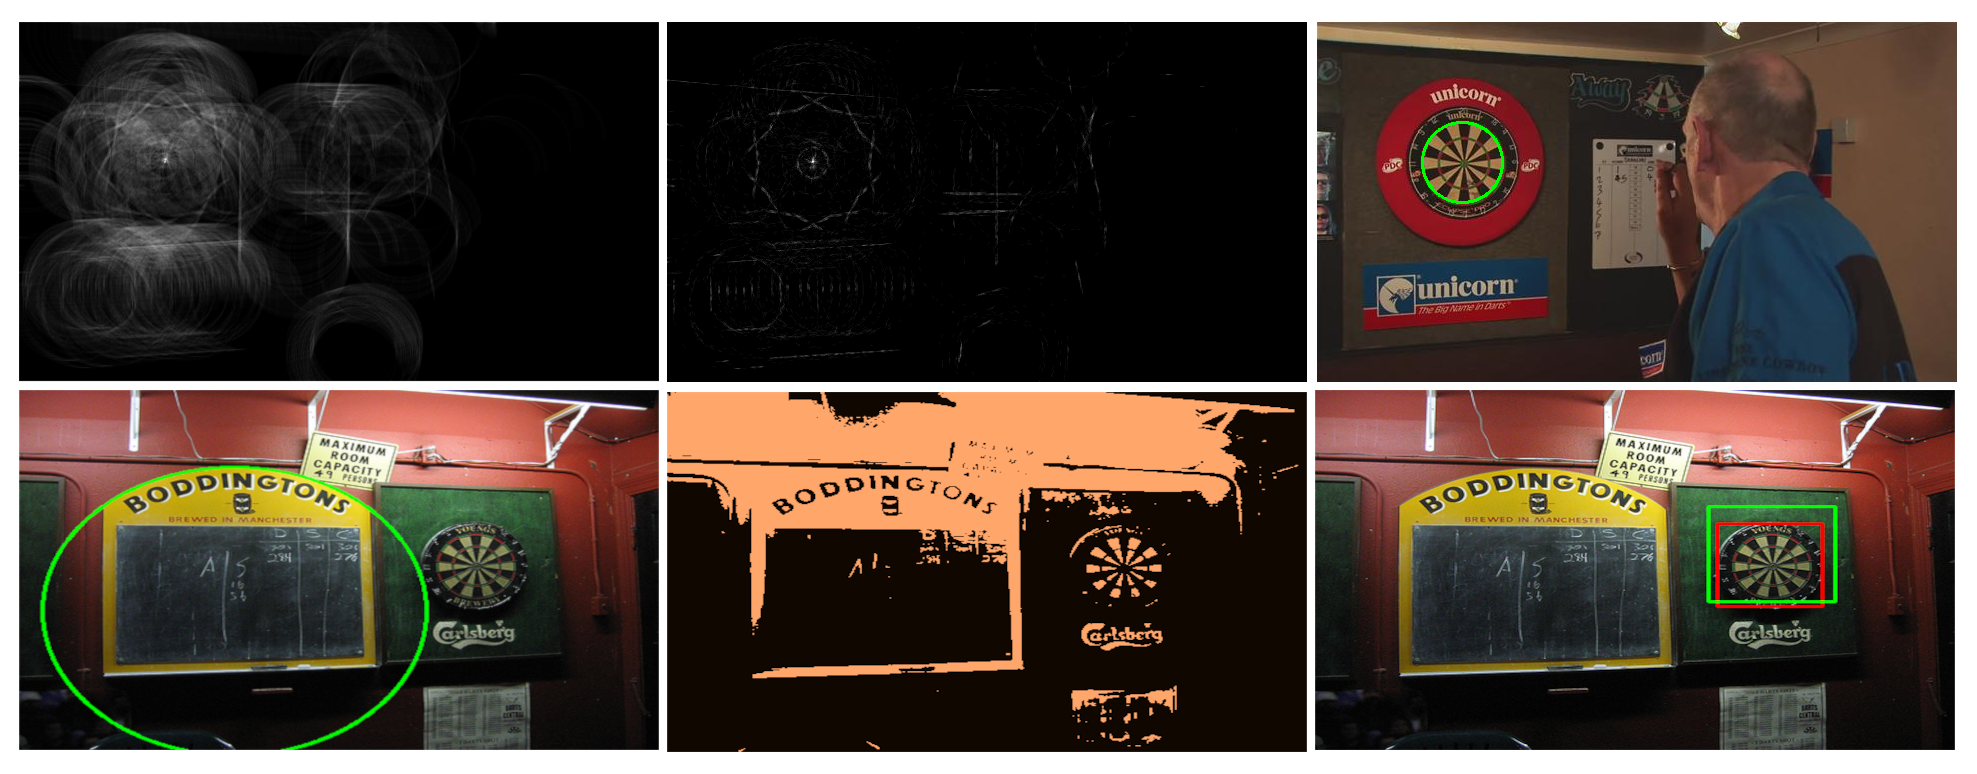
\includegraphics[width=0.95\linewidth]{figures/04_improvements/detector_improvements_images.png}
\caption{Top row $dart2.jpg$: Hough circles space (left), reduced Hough space (middle), TP detected circle (right). Bottom row $dart3.jpg$: FP detected circle (left), KMeans colour segmented (middle), TP detected dartboard (right).}
\label{detector_improvement_images}
\end{figure}

\subsection{Evaluation}

\begin{wraptable}{r}{8cm}
% \begin{table}[h]
\begin{tabular}{|c||c|c|c|} 
    \hline
    Image & Precision & Recall & $F_1$ \\ [0.5ex] 
    \hline
    $dart0$  & 1.00 (+0.00) & 1.00 (+0.00) & 1.00 (+0.00) \\
    $dart1$  & 1.00 (+0.00) & 1.00 (+0.00) & 1.00 (+0.00) \\
    $dart2$  & 0.50 (-0.50) & 1.00 (+0.00) & 0.67 (-0.33) \\
    $dart3$  & 1.00 (+1.00) & 1.00 (+1.00) & 1.00 (+1.00) \\
    $dart4$  & 1.00 (+0.00) & 1.00 (+0.00) & 1.00 (+0.00) \\
    $dart5$  & 0.33 (+0.33) & 1.00 (+1.00) & 0.50 (+0.50) \\
    $dart6$  & 1.00 (+0.00) & 1.00 (+1.00) & 1.00 (+1.00) \\
    $dart7$  & 1.00 (+0.00) & 1.00 (+0.00) & 1.00 (+0.00) \\
    $dart8$  & 0.50 (-0.50) & 0.50 (+0.00) & 0.50 (-0.17) \\
    $dart9$  & 1.00 (+0.50) & 1.00 (+0.00) & 1.00 (+0.33) \\
    $dart10$ & 0.67 (-0.33) & 0.67 (+0.00) & 0.67 (-0.13) \\
    $dart11$ & 0.00 (+0.00) & 0.00 (+0.00) & 0.00 (+0.00) \\
    $dart12$ & 1.00 (+0.00) & 1.00 (+0.00) & 1.00 (+0.00) \\
    $dart13$ & 0.50 (-0.50) & 1.00 (+0.00) & 0.67 (-0.33) \\
    $dart14$ & 0.33 (-0.34) & 1.00 (+0.00) & 0.50 (-0.30) \\
    $dart15$ & 1.00 (+0.00) & 1.00 (+0.00) & 1.00 (+0.00) \\
    \hline\hline
    avg.     & 0.74 (+0.04) & 0.89 (+0.19) & 0.80 (+0.10) \\
    \hline
\end{tabular}
\caption{Dartboard detection performance of final \\ ensemble method with KMeans colour segmentation for each image and overall with improvements over \\ ensemble method shown for each entry.}
\label{final_dartboards_results}
% \end{table}
\end{wraptable} 

% {\color{blue}
% Evaluate your final detector on all of the example images, show the improvements in TPR and $F_1$-score compared to previous approaches. Briefly note in bullet points the key merits and shortcomings of your final implementation.
% } \\

• I aimed to increase the precision of the Viola-Jones method. Final results in Table \ref{final_dartboards_results} show a precision increase 0.22 over the Viola-Jones method whilst retaining high recall, resulting in an $F_1$ of 0.8; an increase of 0.19. Additionally average IoU of detections increased by 22\% over Viola-Jones.

\noindent • Circle detection works well but dartboards are sometimes not straight-on and so are often not circular. Ellipse detection would be a better option for off-centre boards.

\noindent • Lines detection works excellently, but edges are prevalent throughout the image. Using line detection as a method of validating other methods was a good decision.

\noindent • The addition of another shape detector such as triangles would improve recall further whilst retaining precision if added to current ensemble. 

\noindent • Overall my Hough transforms work well and the improvements discussed in \ref{idea_vis} increased precision greatly.

\noindent • KMeans colour segmentation reduced the number of edges in the image reducing FPs.

\noindent • Performance of the system is largely down to parameter selection. Searching the parameter space was limited by the speed of Python, however I have minimised processing time via vectorisation of complex functions. 

\noindent • Greater performance is likely possible but I am pleased with my current implementation and more parameter optimisation would not add further merit to my project.

\end{document}
